\documentclass{article}
\usepackage[utf8]{inputenc}
\usepackage[a4paper, total={6in, 10in}]{geometry}
\usepackage[utf8]{inputenc}
\usepackage{color, colortbl}
\usepackage{graphicx}
\usepackage{multicol}
\usepackage{hyperref}
\usepackage{amsmath}
\usepackage{amssymb}
\usepackage{mathrsfs}
\usepackage{lipsum}
\usepackage{capt-of}
\usepackage{subcaption}
\usepackage{multirow}
\usepackage[most]{tcolorbox}

\begin{document}
\section{Organelle transport with no motors}
\subsection{Viscous media} 
Our starting point is the one-dimensional Langevin equation that describes the time evolution of an organelle, 


\begin{equation}\label{dif}
\gamma_0\dot{x}(t)=\xi_0(t),
\end{equation}

where $x(t)$ is the position of the organelle (also here referred as cargo), $\gamma_0$ is the viscosity of the media, and $\xi_0(t)$ is a Gaussian random noise, here referred as white noise, and which represents the effect of the collisions with the molecules. $\xi_0(t)$ has a Gaussian probability distribution with correlation function

\begin{equation}\label{fluc-disp}
\langle\xi(t) \xi(t')\rangle=k_BT\gamma_0\delta(t-t').
\end{equation}

The viscosity of the media $\gamma_0$ is determined by the Stokes, as $\gamma_0=6\pi R\eta$, where $\eta$ is the viscosity of the media, and $r_o$ is the radius of the cargo. \\

This model represents a purely viscous fluid, in which the resulting cargo displays a diffusive dynamic. Diffusive dynamics are characterized by a Mean Square Displacement (MSD) that satisfies MSD$\sim \Delta t$, in short- and long-term scales. In the models here included we consider $r_o=500$ nm y $k_BT=4.1$ pNnm.

\subsection{Viscoelastic media}

In order to include viscoelastic properties that may result in sub-diffusive regimes, we includes elastic forces between the cargo and $i$ virtual particles described by $x_j(t)$, $j=1\cdots N$. In this way, we consider the effect of cellular crowding. Hence, the movement equation can be written as

\begin{equation}\label{part-virt}
\gamma_0\dot{x}(t)=-\sum_{j=0}^{N-1}k_j(x(t)-x_j(t))+\xi_0(t),                                         \end{equation}

where $k_j$ is the elastic constant associated to the interaction between the cargo and the $j$ virtual particles. Simultaneously, virtual particles satisfy the Langevin equations

\begin{equation}\label{eqspv}
\eta_j\dot{x}_j(t)=k_j(x(t)-x_j(t))+\xi_j(t),
\end{equation}

where $\eta_j$ is the effective viscosity on the virtual particle $j$, and the noise $\xi_j(t)$ satisfy

\begin{equation}\label{fluc-disp2}
\langle\xi_i(t) \xi_j(t')\rangle=k_BT\delta(t-t')\delta_{ij}.
\end{equation}

By defining the frequency and viscosity of the particle $i$ as in:

\begin{gather}\label{def-ctes}
\eta_i=\frac{\gamma_0}{\Gamma(1-\alpha)}\frac{\nu_0^\alpha}{b^{i\alpha}},\hspace{1cm}\nu_i=\frac{\nu_0}{b^i},
\end{gather}

where $\nu_0$ is the maximum frequency, and $b>1$ is a scale paremeter, the equations (\ref{eqspv}-\ref{def-ctes}) can be rewritten as

\begin{align}\label{nu1}
\text{MSD}&\sim(\Delta t)^\alpha  &  &\text{para} & \frac{1}{\nu_0}&<\Delta t<\frac{1}{\nu_{N-1}},
\end{align}
\begin{align}\label{nu2}
\text{MSD}&\sim\Delta t & &\text{para} & \frac{1}{\nu_{N-1}}&<\Delta t.
\end{align}

The values assigned to $\nu_0$ and $N$ generate mixed regimes where, the cargo describes a sub-diffusive dynamic at short time scales, and a diffusive dynamic at long timescales. Figure \ref{regmx} illustrates an example of a mixed regime with a sub-diffusive dynamics of the cargo in $10^{-5}s<\Delta t<10^{-2}$s, but diffusive at $10^{-2}s<\Delta t$ when $N=8$, and $\nu_0=10^{6}$s$^{-1}$, $b=5$.

With $\nu_0$ and $N$ large enough, the resulting mean square displacement satisfies MSD$\sim(\Delta t)^\alpha$ in all time scales. In this case, equations (\ref{part-virt}) and (\ref{eqspv}) are considered as the Markovian approximation of the Generalized Langevin Equation (GLE).

\begin{equation}\label{genlan}
\gamma_0=\xi_0(t)+\int_0^\infty\gamma(t-t')\dot{x}(t')+\xi_\gamma(t),
\end{equation}
con 
\begin{equation}
\gamma(t)=\frac{\gamma_0}{\Gamma(1-\alpha)t^{-\alpha}},
\end{equation}

\begin{figure}[h!]
\centering
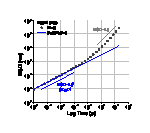
\includegraphics[scale=5]{img/msdmx}
\caption[MSD in mixed regimes as a result of eqs. (\ref{part-virt}) y (\ref{eqspv})]{MSD in mixed regimes as a result of eqs. (\ref{part-virt}) y (\ref{eqspv})}
\label{regmx}
\end{figure}
\end{document}
